\documentclass[a4paper,10pt]{article}
\usepackage[T2A]{fontenc}
\usepackage[utf8]{inputenc}
\usepackage[english,russian]{babel}
\usepackage{circuitikz}
\usepackage{wrapfig}
\usepackage{makecell}
\usepackage{tabularx}
\usepackage{graphicx}
\usepackage{gensymb}
\usepackage{cancel} %cancel symbol
\usepackage{amsmath,amsfonts,amssymb,amsthm,mathtools}
\usepackage{pgfplots}
\usepackage[margin=3cm]{geometry}
\pgfplotsset{compat=1.12}
\usepackage{mathrsfs}
\usepackage{multirow}
\usepackage[table,xcdraw]{xcolor}
\usepackage{tabto}
%tikz (draw)

\usepackage{tikz}
\usepackage{pstricks-add}
%tikz libraries

\usetikzlibrary{intersections}
\usetikzlibrary{arrows.meta}
\usetikzlibrary{calc,angles,positioning}
\usetikzlibrary{arrows}
\usepackage{float}

\parindent=0ex % красная строка (ее отсутсвие)

\graphicspath{ {C:/Users/Admin/Documents/TEX/test} }


\begin{document}
    \begin{center}
        МОСКОВСКИЙ ГОСУДАРСТВЕННЫЙ УНИВЕРСИТЕТ \\
        ИМ. М.В. ЛОМОНОСОВА \\
        
        
        \hfill \break
        Факультет вычислительной математики и кибернетики\\
        \vspace{2.5cm}
        \Large{\textbf{Отчет по заданию № 1}}\\
        \vspace{0.5cm}
        \large{\textbf{<<Методы сортировки>>}}\\
        \vspace{0.5cm}
        \large{\textbf{Вариант 3 3 2 4}}\\
        \hfill \break
        \\
    \end{center}
    \begin{flushright}
        \textbf{Исполнитель:}\\ 
        Студент гр. 106\\
        Кондрашов Д.С.\\
        \vspace{0.2 cm}
        \textbf{Преподаватели:}\\ 
        Корухова Л.С.\\ 
        Манушин Д.В. \\

    \end{flushright}
    \vfill

    \begin{center}
        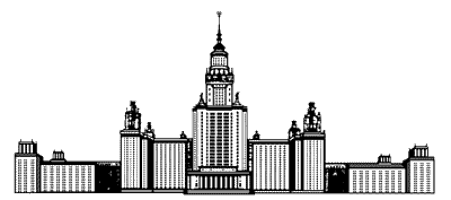
\includegraphics[width = 0.5\linewidth] {msu_logo}
    \end{center}
    \begin{center} 
        Москва, 2024 
    \end{center}
	\thispagestyle{empty} %отсутсвие нумерации на странице

    \newpage
    \tableofcontents %оглавление

    \thispagestyle{empty} %отсутсвие нумерации на странице

    \newpage
    \pagenumbering{arabic} % тип последующей нумерации 
    \section{Постановка задачи}
    \vspace{0,5cm}
    \textbf{1.} Требуется реализовать два метода сортировки одномерного массива: \\
    \hspace*{1 cm} 1) Сортировка методом простого выбора \\
    \hspace*{1 cm} 2) Быстрая сортировка, основанная на рекурсивной реализации\\ 
    \hspace*{1.2 cm} \textit{(Числа упорядочиваются по неубыванию модулей)}\\
    \textbf{2.} Сравнить асимптотическую сложность данных алгоритмов. \\
    \textbf{3.} На основе полученных результатов предоставить таблицу сравнений и сделать вывод.
    \vspace{1.3cm}

    %\newpage
    \section{Результаты экспериментов}
    \vspace{0.3cm}
    В результате проведенных экспериментов была подтверждена асимптотическая сложность алгоритмов:
    \begin{center}
        Selection sort  $O(n\cdot(n-1)/2)$ \\
        Quick sort  $O(n\cdot\log_2n)$\\
    \end{center}
    

    
    \begin{table}[H]
        \begin{tabular}{ccccccl}
                                                                &                                             & \textbf{1}           & \textbf{2}           & \textbf{3}           &                                             &  \\
        \multirow{-2}{*}{\textit{\textbf{N}}}                   & \multirow{-2}{*}{\textbf{Номер сортировки}} & \multicolumn{1}{l}{} & \multicolumn{1}{l}{} & \multicolumn{1}{l}{} & \multirow{-2}{*}{\textbf{Среднее значение}} &  \\
        {\color[HTML]{3F3B42} }                                 & Сравнения                                   & 45,00                & 45,00                & 45,00                & 45,00                                       &  \\
        \multirow{-2}{*}{{\color[HTML]{3F3B42} \textbf{10}}}    & Перемещения                                 & 6,82                 & 6,80                 & 6,99                 & 6,87                                        &  \\
        {\color[HTML]{3F3B42} }                                 & Сравнения                                   & 1 225,00             & 1 225,00             & 1 225,00             & 1 225,00                                    &  \\
        \multirow{-2}{*}{{\color[HTML]{3F3B42} \textbf{50}}}    & Перемещения                                 & 45,47                & 45,19                & 45,67                & 45,45                                       &  \\
        {\color[HTML]{3F3B42} }                                 & Сравнения                                   & 4 950,00             & 4 950,00             & 4 950,00             & 4 950,00                                    &  \\
        \multirow{-2}{*}{{\color[HTML]{3F3B42} \textbf{100}}}   & Перемещения                                 & 94,89                & 94,62                & 94,50                & 94,67                                       &  \\
        {\color[HTML]{3F3B42} }                                 & Сравнения                                   & 124 750,00           & 124 750,00           & 124 750,00           & 124 750,00                                  &  \\
        \multirow{-2}{*}{{\color[HTML]{3F3B42} \textbf{500}}}   & Перемещения                                 & 492,40               & 493,14               & 493,70               & 493,08                                      &  \\
        {\color[HTML]{3F3B42} }                                 & Сравнения                                   & 499 500,00           & 499 500,00           & 499 500,00           & 499 500,00                                  &  \\
        \multirow{-2}{*}{{\color[HTML]{3F3B42} \textbf{1000}}}  & Перемещения                                 & 992,10               & 992,40               & 992,30               & 992,27                                      &  \\
        {\color[HTML]{3F3B42} }                                 & Сравнения                                   & 12 497 500,00        & 12 497 500,00        & 12 497 500,00        & 12 497 500,00                               &  \\
        \multirow{-2}{*}{{\color[HTML]{3F3B42} \textbf{5000}}}  & Перемещения                                 & 4 990,35             & 4 990,40             & 4 991,20             & 4 990,65                                    &  \\
        {\color[HTML]{3F3B42} }                                 & Сравнения                                   & 49 995 000,00        & 49 995 000,00        & 49 995 000,00        & 49 995 000,00                               &  \\
        \multirow{-2}{*}{{\color[HTML]{3F3B42} \textbf{10000}}} & Перемещения                                 & 9 989,10             & 9 989,60             & 9 990,59             & 9 989,76                                    & 
        \end{tabular}
    \end{table}
    \vspace{0.3cm}
    ** количество массивов  было сокращено с 4 до 3, потому что каждое полученное число - это среднее из 10000 прогонов с различными массивами одной длинны\\

    \textbf{1} - элементы упорядочены, \\ 
    \textbf{2} - элементы упорядочены в обратном порядке,\\ 
    \textbf{3} - расстановка элементов случайна\\
    

    \vspace{0.8cm}
    \large{\textbf{Вывод:}}\\
    В результате проведеных опытов были подтверждены формулы, использующиеся для нахождения асимптотической сложности алгоритмов, и было сделано заключение о том, что quick sort быстрее, чем selection sort, но для этого нужны наиболее случайные значения, при росте количества элементов массива эта разница становится заметнее еще больше.


    \newpage
    \section{Структура программы и спецификация функций}
    \vspace{0,5cm}
    Для более оптимизированной работы программы использовались функции, которые работали как с массивом данных, так и с численными перменными.
    \vspace{0.5cm}\\
    \textbf{Список функций:}\\
    \begin{enumerate}
        \item change() -- функция меняет местами два элемента массивов, которые ей подаются.
        \item selection\_sort() -- функция сортирует массив методом выбора и подсчитывает количество изменений и сравнений, которые были при этом сделаны.
        \item fast\_sort() -- функция сортирует массив методом быстрой сортировки рекурсией и подсчитывает количество изменений и сравнений, которые были при этом сделаны.
        \item sort\_q() -- сортирует массив по возрастанию, используя алгоритм selection sort.
        \item sort\_rev() -- сортирует массив в обратнмо порядке, используя алгоритм selection sort.
        \item filling() -- заполняет массив случайным числами, используя условие, которое было выбрано.
        \item sred() -- подсчитывает среднее из всех элементов массива
    \end{enumerate}
    \newpage
    \section{Отладка программы, тестирование программы}
    \vspace{0,5cm}
    Для отладки и соотвествующей тестировки программы в каждую из сортирующий функций был добавлен вывод массива после каждого прохода по нему.\\ 
    (Далее будет представлен пример прохода по случайному массиву и его сортировка)\\
    
    \textbf{selection\_sort} \\
    \vspace{0.1cm}\\
    172.00\qquad 5992.90\qquad -4900.79\qquad -7914.01\qquad 24101.29\qquad 5888.81\qquad 
    -12516.97\qquad \\
    172.00\qquad -4900.79\qquad 5992.90\qquad -7914.01\qquad 24101.29\qquad 5888.81\qquad 
    -12516.97\qquad \\
    172.00\qquad -4900.79\qquad 5888.81\qquad -7914.01\qquad 24101.29\qquad 5992.90\qquad 
    -12516.97\qquad \\
    172.00\qquad -4900.79\qquad 5888.81\qquad 5992.90\qquad 24101.29\qquad -7914.01\qquad 
    -12516.97\qquad \\
    172.00\qquad -4900.79\qquad 5888.81\qquad 5992.90\qquad -7914.01\qquad 24101.29\qquad 
    -12516.97\qquad \\
    172.00\qquad -4900.79\qquad 5888.81\qquad 5992.90\qquad -7914.01\qquad -12516.97\qquad 24101.29\qquad \\
    
    \vspace{0.1cm}
    \textbf{quick\_sort} \\
    \vspace{0.1cm}\\
    172.00\qquad 5992.90\qquad -4900.79\qquad 5888.81\qquad 24101.29\qquad -7914.01\qquad -12516.97\qquad \\ 
    172.00\qquad -4900.79\qquad 5992.90\qquad 5888.81\quad | \quad-7914.01\qquad 24101.29\qquad -12516.97\qquad \\ 
    172.00\qquad -4900.79\quad | \enspace5888.81\qquad5992.90\quad|\quad-7914.01\quad|\quad-12516.97 \quad24101.29\qquad \\ 
    
    \vspace{0.5cm}
    \small{P.S. при проверке отсортированного массива не стоит забывать, что элементы сорртируются по неубыванию модулей}
    \vspace{1.5cm}

    \section{Анализ допущенных ошибок}
    \vspace{0,5cm}
    При написании функции 
    \textbf{fast\_sort()} для сортировки массива методом быстрой сортировки (рекурсивная реализация), была допущена ошибка: \\
    значение pivot (опорного элемента) сохранялось, как значение индекса этого элемента в массиве, а не как вещественное число, из-за чего при выполнение функции значение pivot могло меняться в течение одного прохода, что привело к неправильной сортировке массивов.   


    \newpage
    \section{Литература}
    \vspace{0.5cm}

    \begin{thebibliography}{10}
        \vspace{0.5cm}
        \bibitem{}
        Трифонов Н. П., Пильщиков В. Н. Задания практикума на ЭВМ (1 курс). Методическая разработка(составители). — М.: ВМК МГУ, 2001.
        \bibitem{}
        Кормен Т., Лейзерсон Ч., Ривест Р., Штайн К. Алгоритмы: построение и анализ. Второе издание.
        — М.: «Вильямс», 2005.
        \bibitem{}
        Головинов Г.  Основы программирования на TeX. Том 1. Начало. — М.: МФТИ, 2024.
        \bibitem{}
        Кнут Д. Искусство программирования для ЭВМ. Том 3. — М.: Мир, 1978.
        \bibitem{}
        Лорин Г. Сортировка и системы сортировки. — М.: Наука, 1983.
    \end{thebibliography}

    


\end{document}

